\newpage

\section{Вычислительный эксперимент}

\textbf{Выборка FashionMNIST.} Эксперимент проводился для задачи классификации для выборки FashionMNIST~\cite{FMNIST}. В качестве модели учителя \textbf{f} рассматривается четырёхслойная нейросеть, в качестве функции активации рассматривается ReLu. В качестве модели ученика рассматривается однослойная нейросеть.\\
На рисунках 1, 2 показаны графики зависимостей Accuracy и кросс-энтропии на тестовой выборке между истинными метками объектов и вероятностями, предсказанными моделью ученика. На графиках видно, что модель, использующая метки учителя, показывает лучшее значение Accuracy, но большее значение ошибки.

\begin{figure}[h!t]\center
\subfloat[]
{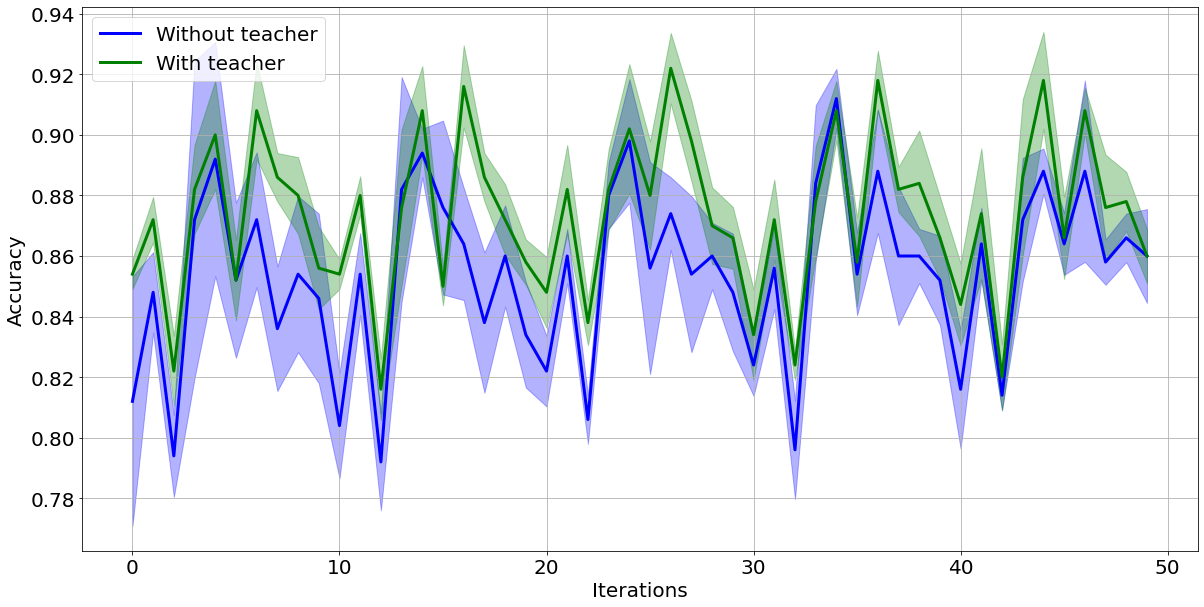
\includegraphics[width=0.5\textwidth]{results/accuracy}}
\subfloat[]
{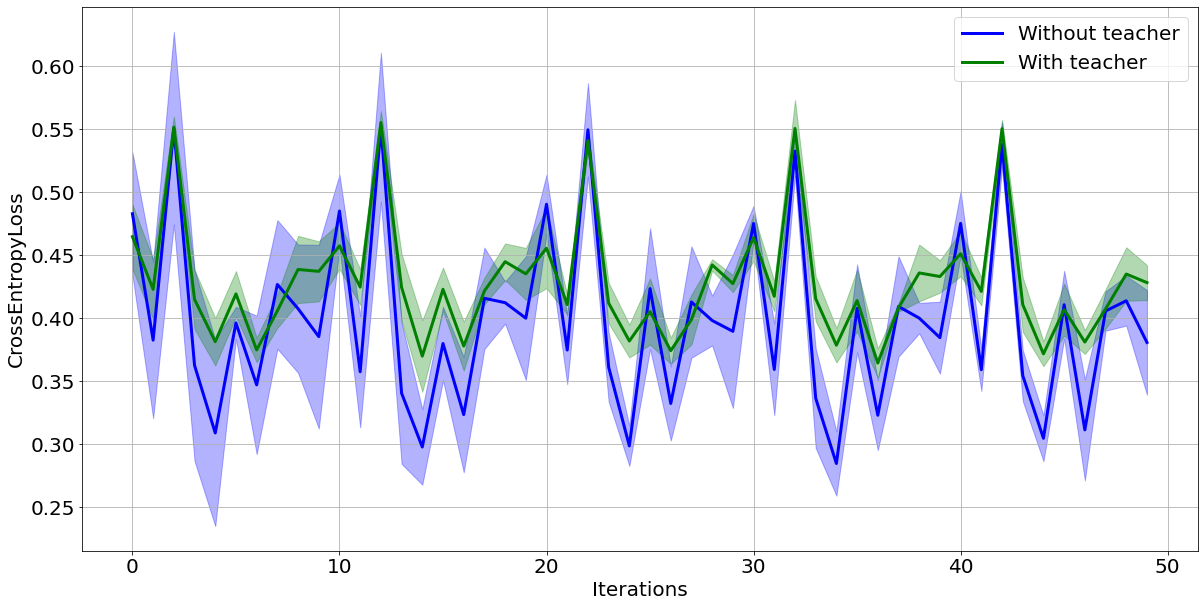
\includegraphics[width=0.5\textwidth]{results/loss}}\\
\caption{Зависимость a) Accuracy; b) CrossEntropyLoss между истинными и предсказанными учеником метками от числа итераций на тестовой выборке}
\end{figure}


\newpage
\subsection{Базовый экперимент}
